\documentclass[aspectratio=169]{beamer}

\usepackage[hyperref,backend=biber,
% Exemples de styles: alphabetic, ieee, nature, numeric, verbose-trad1 (en utilisant \footcite{}).
% https://www.overleaf.com/learn/latex/Biblatex_bibliography_styles
style=alphabetic,
% backref=true,
% backrefstyle=three,
]{biblatex}

\newif\ifwebcast
\webcastfalse
\newcommand{\webcast}{\webcasttrue}
% \webcast
% \newcommand<>{\script}[1]{\note#2{{#1}}}
% \newcommand<>{\script}[1]{\note{\only#2{#1}}}
\def\script{\note}

\definecolor{supelecRed}{RGB}{120,30,56}
\definecolor{supelecPurple}{RGB}{104,95,115}
\usetheme{Thesis}

\usepackage[utf8]{inputenc}
\usepackage[english]{babel}
\usepackage{tikz}
\usepackage{bm}
\usepackage{ulem}
\usepackage{parcolumns}
\usepackage{multicol}
\usepackage{booktabs}
\usepackage[french]{isodate}
\usepackage[ruled,noend,algo2e]{algorithm2e}
\usepackage[T1]{fontenc}
\usepackage{lmodern} % Assurer une bonne impression!
\usepackage{tikz} % tikz est utilise pour tracer des boites, par exemple
\usepackage{pgfplots}
\usepackage{fix-cm}
\usepackage{grffile}
\usepackage{pgfpages}
\usepackage{xparse}

\usepackage{pifont} % Pour utiliser des symboles divers.
\usepackage{color}
\usepackage{comment}
\usepackage{xargs}
\usepackage[author={Accacio}]{pdfcomment}

\usepackage{mathtools}
\usepackage{amsmath}
\usepackage{amsthm}
\usepackage{mathrsfs}
\usepackage{mathbbol}

\usepackage{eucal}

\usepackage{subcaption}
\usepackage{caption}
\captionsetup{justification=centering}
\usepackage{float}
\usepackage{array}

\usepackage{xr}
\usepackage{subfiles}
\usepackage[math]{blindtext}
\usepackage{ifthen} % Entrer valeurs bool\'{e}ennes et autres options
\usepackage{csquotes} % Assurer les guillemets français

\usepackage{nicefrac,xfrac}
\usepackage{etoolbox}
\usepackage{fontawesome}
\usepackage{mathabx}

\usepackage{animate}
\usepackage{colortbl}

\definecolor{mpc_agent}{RGB}{243, 146, 0} % logo necsys
\colorlet{mpc_agent}{supelecRed!90}
\definecolor{mpc_coordinator}{RGB}{235, 235, 235}
\colorlet{mpc_coordinator}{supelecRed!10}
\definecolor{mpc_green}{RGB}{98, 160, 98}
\newcommand\encircle[1]{%
  {
  \usebeamerfont*{item projected}%
  \usebeamercolor[bg]{item projected}%
  \begin{pgfpicture}{-1ex}{0ex}{1ex}{2ex}
    \pgfpathcircle{\pgfpoint{0pt}{.75ex}}{1.4ex}
    \pgfusepath{fill}
    \pgftext[base]{\color{fg}#1}
  \end{pgfpicture}%
  }
}

\newcommand{\tikzmark}[1]{\tikz[baseline={(#1.base)},overlay,remember picture] \node[outer sep=0pt, inner sep=0pt] (#1) {\phantom{A}};}

\newcommand{\booksymbol}{\lower4pt\hbox{\pgfuseimage{beamericonbook}}}
\tikzset{%
  show controls/.style={
    postaction={
      decoration={
        show path construction,
        curveto code={
          \draw [blue]
          (\tikzinputsegmentfirst) -- (\tikzinputsegmentsupporta)
          (\tikzinputsegmentlast) -- (\tikzinputsegmentsupportb);
          \fill [red, opacity=0.5]
          (\tikzinputsegmentsupporta) circle [radius=.2ex]
          (\tikzinputsegmentsupportb) circle [radius=.2ex];
        }
      },
      decorate
    }}}

\usetikzlibrary{graphs,quotes,graphs.standard}
\usetikzlibrary{plotmarks}
\usetikzlibrary{arrows.meta}
\usepgfplotslibrary{patchplots}
\usetikzlibrary{calc,shapes,positioning}
\usetikzlibrary{math}
\usetikzlibrary{overlay-beamer-styles}
\tikzset{
  graphs/nodes={draw,circle,inner sep=1pt},
  <->/.style={latex-latex},
  ->/.style={-latex},
  <-/.style={latex-},
}
\usetikzlibrary {chains}
\usetikzlibrary{arrows.meta}
\usetikzlibrary{3d}
\usetikzlibrary{perspective}
\usetikzlibrary{calc,shapes,positioning,intersections}
\usetikzlibrary{overlay-beamer-styles}
 \usetikzlibrary{plotmarks}
  \usetikzlibrary{arrows.meta}
\usetikzlibrary{babel} % to correct problem with babel

% \usepackage{times}
% Or whatever. Note that the encoding and the font should match. If T1
% does not look nice, try deleting the line with the fontenc.
\graphicspath{{../img/}}

\usepackage{amssymb}
\usepackage{accents}

\SetKwRepeat{Do}{do}{while}


\newcommand{\eq}[2]{\mbox{$#1=#2$}}
\newcommand{\N}{\mathbb{N}}
\newcommand{\Z}{\mathbb{Z}}
\newcommand{\Q}{\mathbb{Q}}
\newcommand{\R}{\mathbb{R}}
\newcommand{\C}{\mathbb{C}}
\newcommand{\Np}{N_{\text{p}}}
\newcommand{\T}{^{\mathrm{T}}}
\newcommand{\1}{\mathbf{1}}
\newcommand{\0}{\mathbf{0}}
\newcommand{\abs}[1]{\left\lvert#1\right\rvert}
\newcommand{\norm}[1]{\left\lVert#1\right\rVert}
\newcommand{\blkdiag}{\mathop{\rotatebox{90}{$\diameter$}}}

\newcommand{\vectorize}[1]{\mathrm{vec} (#1)}
\newcommand{\Varepsilon}{\mathcal{E}}
\newcommand{\diff}{\mathop{}\mathopen{}\mathrm{d}}
\newcommand{\set}[1]{\mathcal{#1}}
\newcommand{\graph}[1]{\mathscr{#1}}
\newcommand{\p}{^{(p)}}
\newcommand{\pplusone}{^{(p+1)}}
\newcommand{\h}{^{(h)}}
\newcommand{\hplusone}{^{(h+1)}}
\renewcommand{\vec}[1]{\boldsymbol{#1}}
\newcommand{\random}[1]{\underline{#1}}
\newcommand{\randomvec}[1]{{\underline{\vec{#1}}}}
\newcommand{\probability}[1]{\mathbb{P}(#1)}
\newcommand{\pdf}[1]{p(#1)}
\newcommand{\expectation}[2][]{\mathbb{E}_{#1}\left[#2\right]}
\newcommand{\indicator}[1]{\mathbb{1}_{\{#1\}}}
\newcommand{\vecangle}[2]{\langle_{#1}^{#2}}
\newcommand{\until}{\mathbin{:}}
\newcommand{\pseudoinv}[1]{{#1}^{\dagger}}


\newcommand{\setbuild}[2]{\{#1\mid#2\}}
\newcommand{\seq}[2][n]{\lbrace #2_{0},\ldots,\,#2_{#1} \rbrace}
\newcommand{\hadamard}[2]{#1\circ #2}
\newcommand{\kron}[2]{#1\otimes#2}
\newcommand{\symmetric}{\mathbb{S}}
\newcommand{\semidefpos}{\mathbb{S}_{+}}
\newcommand{\defpos}{\mathbb{S}_{++}}
\newcommand{\elem}[2][1]{{#2}_{(#1)}}
\renewcommand{\implies}{\Rightarrow}
\renewcommand{\iff}{\Leftrightarrow}
\newcommand{\argmax}{\mathop{\arg\!\max}}
\newcommand{\argmin}{\mathop{\arg\!\min}}
\newcommand{\maximize}{\mathop{\textrm{maximize}}}
\newcommand{\minimize}{\mathop{\textrm{minimize}}}
\newcommand{\minimiser}{\mathop{\textrm{minimiser}}}
\newcommand{\maximiser}{\mathop{\textrm{maximiser}}}

\DeclareMathOperator{\elemend}{end}
\DeclareMathOperator{\diag}{diag}
\DeclareMathOperator{\fix}{fix}
\DeclareMathOperator{\Proj}{Proj}
\DeclareMathOperator{\dom}{dom}
\DeclareMathOperator{\card}{\#}
% \DeclareMathOperator{\vectorize}{vector}
% \DeclareMathOperator{\vector}{vec}
%

% Theorem
% \newtheorem{thm}{Theorem}[section]
% \newtheorem{lem}[thm]{Lemma}

\newcommand{\nsubsystems}{M}
\newcommand{\umax}{\vec{u}_{\mathrm{\max}}}
\newcommand{\predhorz}{N}
\newcommand{\predictionSet}{\set{N}}
\newcommand{\nineq}{n_{\text{ineq}}}

\NewDocumentCommand \mpcvec { s m o o o } {%
  \IfBooleanTF{#1}{
    \def\optim{^\star}
  }{
    \def\optim{}
  }
  \IfValueTF{#5}{
    \vec{#2}_{#3}\optim{}[#4|#5]
  }{
    \IfValueTF{#4}{
      \vec{#2}_{#3}\optim{}[#4]
    }
    {
    \IfValueTF{#3}{
      \vec{#2}_i\optim{}[#3]
    }
    {
      \vec{#2}_i\optim{}[k]
    }
    }
  }
}


\NewDocumentCommand \mpcval { s m o o o } {%
  \IfBooleanTF{#1}{
    \def\optim{^\star}
  }{
    \def\optim{}
  }
  \IfValueTF{#5}{
    {#2}_{#3}\optim{}[#4|#5]
  }{
    \IfValueTF{#4}{
      {#2}_{#3}\optim{}[#4]
    }
    {
    \IfValueTF{#3}{
      {#2}_i\optim{}[#3]
    }
    {
      {#2}_i\optim{}[k]
    }
    }
  }
}






\newcommand{\uikk}{\mpcvec{u}[i][k][k]}
\newcommand{\optuikk}{\mpcvec*{u}[i][k][k]}

\newcommand{\globobj}{\mpcval{J}[][k]}
\newcommand{\optglobobj}{\mpcval*{J}[][k]}

\newcommand{\eqobj}{\bar{J}}
\newcommand{\eqoptobj}{\eqobj^{\star}}
\newcommand{\eqobji}{\eqobj_{i}}
\newcommand{\eqoptobji}{\eqobj_{i}^{\star}}
\newcommand{\obj}{J}
\newcommand{\optobj}{\obj^{\star}}
\newcommand{\obji}{\obj_{i}}
\newcommand{\optobji}{\obj_{i}^{\star}}
\newcommand{\Jacc}{\obj^{\text{acc}}}
\newcommand{\Jiacc}[1][i]{\obj_{#1}^{\text{acc}}}


\newcommand{\xik}{\mpcvec{x}}
\newcommand{\fik}{\mpcvec{f}}
\newcommand{\uik}{\mpcvec{u}}
\newcommand{\uiseq}{\mpcvec{u}[i][k:k+\predhorz-1][k]}
\newcommand{\optuiseq}{\mpcvec*{u}[i][k:k+\predhorz-1][k]}

\newcommand{\useq}{\mpcvec{u}[ ][k:k+\predhorz-1][k]}
\newcommand{\optuseq}{\mpcvec*{u}[ ][k:k+\predhorz-1][k]}
\newcommand{\Uik}{\mpcvec{U}}
\newcommand{\optUik}{\mpcvec*{U}}
\newcommand{\optuncUik}{\mpcvec*{\mathring{U}}}
\newcommand{\optuncU}{{\mathring{\vec{U}}^{\star}}}

\newcommand{\vik}{\mpcvec{v}}
\newcommand{\wik}{\mpcvec{w}}
\newcommand{\wiseq}{\mpcvec{w}[i][k:k+\predhorz-1][k]}
\newcommand{\Wik}{\mpcvec{W}}

\newcommand{\qik}{\mpcvec{q}}
\newcommand{\qiseq}{\mpcvec{q}[i][k:k+\predhorz-1][k]}
\newcommand{\thetaik}{\mpcvec{\theta}}
\newcommand{\optthetaiseq}{\mpcvec*{\theta}[i][k:k+\predhorz-1][k]}
\newcommand{\thetaseq}{\mpcvec{\theta}[][k:k+\predhorz-1][k]}
\newcommand{\optthetaseq}{\mpcvec*{\theta}[][k:k+\predhorz-1][k]}
\newcommand{\thetai}[1][i]{\vec{\theta}_{#1}}
\newcommand{\optthetai}{\vec{\theta}_i^{\star}}

\newcommand{\dik}{\mpcvec{d}}
\newcommand{\diseq}{\mpcvec{d}[i][k:k+\predhorz-1][k]}
\newcommand{\lambdaik}{\mpcvec{\lambda}}
\newcommand{\lambdaikstar}{\mpcvec*{\lambda}}
\newcommand{\lambdai}[1][i]{\vec{\lambda}_{#1}}
% \newcommand{\modified}[1]{\underaccent{\sim}{#1}}
\newcommand{\modified}[1]{\accentset{\text{mod}}{#1}}
\newcommand{\reconstructed}[1]{\accentset{\text{rec}}{#1}}
\newcommand{\lambdaimodified}{\modified{\vec{\lambda}}_{i}}
\newcommand{\lambdamodified}{\modified{\vec{\lambda}}}
\newcommand{\lambdaireconstructed}{\reconstructed{\vec{\lambda}}_{i}}
\newcommand{\lambdaicheat}{\tilde{\vec{\lambda}}_{i}}
\newcommand{\thetairestricted}{\overset{\scalebox{.5}{$\diameter$}}{\thetai}}

% \newcommand{\Tik}{\mpcval{T}}
\newcommand{\Tik}[1][i]{T_{#1}[k]}
\newcommand{\Tikinvestimate}[1][i]{\widehat{\Tik[#1]^{-1}}}
\newcommand{\Plin}[1][i]{{P}_{#1}}
\newcommand{\Plinnominal}[1][i]{\bar{{P}}_{#1}}
\newcommand{\Plintilde}[1][i]{\tilde{P}_{#1}[k]}
\newcommand{\Plintildeestimate}[1][i]{\widehat{\tilde{P}}_{#1}[k]}
\newcommandx*\Plinineq[2][1=i, 2=0]{\Plin[#1]^{\left(#2\right)}}
\newcommandx*\Plinineqnominal[2][1=i, 2=0]{\bar{\Plin[#1]}^{\left(#2\right)}}
\newcommandx*\Plinineqtilde[2][1=i, 2=0]{\widetilde{\Plin[#1]}^{\left(#2\right)}}
\newcommandx*\Plinineqtildeestimate[2][1=i, 2=0]{\widehat{\widetilde{\Plin[#1]}}^{\left(#2\right)}[k]}

\newcommand{\sik}[1][i]{\vec{s}_{#1}[k]}
\newcommand{\siktilde}[1][i]{\tilde{\vec{s}}_{#1}[k]}
\newcommand{\siktildeestimate}[1][i]{\widehat{\tilde{\vec{s}}}_{#1}[k]}
\newcommandx*\sikineq[2][1=i, 2=0]{\vec{s}_{#1}^{\left(#2\right)}[k]}
\newcommandx*\sikineqtilde[2][1=i, 2=0]{\widetilde{\vec{s}_{#1}}^{\left(#2\right)}[k]}
\newcommandx*\sikineqtildeestimate[2][1=i, 2=0]{\widehat{\widetilde{\vec{s}_{#1}}}^{\left(#2\right)}[k]}

\newcommand{\lagrangianname}{\mathscr{L}}
\newcommand{\lagrangian}{\lagrangianname(\vec{U}_{i}[k],\lambdaik,\thetaik)}
\newcommand{\dualfunctionname}{\mathscr{D}}
\newcommand{\dualfunction}{\dualfunctionname(\lambdaik,\thetaik)}
\newcommand{\inequalityfunctionname}{g_i}
\newcommand{\inequalityfunction}{\inequalityfunctionname(\vec{U}_{i}[k],\thetaik)}
\newcommand{\equalityfunctionname}{h_i}
\newcommand{\equalityfunction}{\equalityfunctionname(\vec{U}_{i}[k],\thetaik)}
\newcommand{\linearcoefi}{\bar{\Gamma}_{i}H_{i}^{-1}\bar{\Gamma_{i}}^{T}}
\newcommand{\linearcoefiineqnonzero}[1][\star,\star]{\elem[#1]{\bar{\Gamma}_{i}}H_{i}^{-1}{(\elem[#1]{\bar{\Gamma}_{i}})}^{T}}

\newcommand{\rlsparam}{{\vec{\nu}_{i}}}
\newcommand{\rlssysinput}{{B_i}}
\newcommand{\rlssysoutput}{{\lambdai}}
\newcommand{\rlsgain}{{\Phi}}
\newcommand{\rlsforget}{{\phi}}
\newcommand{\rlsresidual}{{\epsilon}}

\newcommand{\pwaestparam}{{\vec{\nu}}}
\newcommand{\pwaestnumparam}{{n}}
\newcommand{\pwaestsysinput}{{B}}
\newcommand{\pwaestsysoutput}{{\vec{\gamma}}}
\newcommand{\pwaestgain}{{\Phi}}
\newcommand{\pwaestforget}{{\phi}}
\newcommand{\pwaestresidual}{{\epsilon}}
\newcommand{\pwaestinputsize}{{N}}


\SetKwProg{Fn}{}{}{}
\SetKwFunction{structDataSym}{structDataSym}%
\SetKwBlock{coordinit}{ Coordinator initialization:}{}
\SetKwBlock{exchange}{ Exchange between Coordinator and agents:}{}
\SetKwBlock{negotPhase}{ Negotiation Phase:}{}
\SetKwBlock{detectPhase}{ Detection Phase:}{}

\SetKwBlock{coordinitfr}{ Initialisation du Coordinateur:}{}
\SetKwBlock{exchangefr}{ Échange entre Coordinateur et agents:}{}
\SetKwBlock{negotPhasefr}{ Phase de Négociation:}{}
\SetKwBlock{detectPhasefr}{ Phase de Détection:}{}
\SetKwIF{Si}{SinonSi}{Sinon}{si}{alors}{sinon si}{sinon}{}
\SetKwFor{Tq}{tant que}{faire}{fintq}
\SetKwRepeat{Repeter}{répéter}{jusqu’à}
\SetKwInput{Entree}{Entrées}
\SetKwInput{Sortie}{Sorties}


\newtheorem{assumption}{Assumption}%[numberby]
\newtheorem{assumptions}[assumption]{Assumptions}
\newtheorem{remark}{Remark}

\newif\ifdebug%
\newcommand{\draft}{\debugtrue}
\newcommand{\final}{\debugfalse}
\newcommand{\todo}[2][FORGOT TO DO SOMETHING]{\ifdebug%
  {%
    \color{red}
    #2}\else \PackageError{}{#1}{#2}#2\fi}%
\newcommand\doing[2][FORGOT TO DO SOMETHING]{\ifdebug%
  {%
    \color{blue}
    #2}\else \PackageError{}{#1}{#2}#2\fi}%
\newcommand\warning[1]{\ifdebug%
  {%
    \color{red}
    #1}\fi}

% \setbeameroption{show notes on second screen}
% \webcast
\setbeamercolor{alerted text}{fg=supelecRed}
\bibliography{../tex/bibliography.bib}
\title[Security of dMPC under False Data injection] % (optional, use only with long paper titles)
{Security of distributed Model Predictive Control\\ under False Data injection}

\subtitle
{or How I Learned to Stop and Worry about Everything}

\author[Rafael Accácio Nogueira] % (optional, use only with lots of authors)
{Rafael Accácio NOGUEIRA}

\institute[IETR --- CentraleSupélec] % (optional, but mostly needed)
{
}

\day12 \month12 \year2022
\date[2022-12-12] % (optional, should be abbreviation of conference name)
{
  \today\\
  \begin{minipage}{.3\textwidth}
    \centering
    
\includegraphics[width=2cm]{logos/IETR_2022.png}
  \end{minipage}
  \hfill
  \begin{minipage}{.3\textwidth}
    \centering
    \vspace{10pt}
    
\includegraphics[width=1.5cm]{qrPresentation.png}
    % qrencode https://github.com/Accacio/thesis/raw/main/presentation/presentation.pdf -o ~/git/SysTol21/img/qrPresentation.png
    \href{https://bit.ly/3g3S6X4}{https://bit.ly/3g3S6X4}
  \end{minipage}
  \begin{minipage}{.3\textwidth}
    \centering
    \vspace{10pt}
    
\includegraphics[width=2cm]{logos/supelec.jpeg}
  \end{minipage}
}
% - Either use conference name or its abbreviation.
% - Not really informative to the audience, more for people (including
%   yourself) who are reading the slides online

\subject{}

\logo{
\includegraphics[width=1.5cm]{logos/supelec.jpeg}}

% Delete this, if you do not want the table of contents to pop up at
% the beginning of each subsection:
\AtBeginSection[]
{
  \begin{frame}<beamer>{Outline}
    \tableofcontents[sectionstyle=show/hide,subsectionstyle=show/show/hide]
  \end{frame}
}

\begin{document}

\begin{frame}[plain]
  % \frametitle{Ph.D. Defense}
  \titlepage%
  \note{45 minutes !!!!\\}
  \script{Hello, I'm Rafael Accácio}
  \script{This presentation is available at the address shown or by flashing the QR code.\\}
\end{frame}

\begin{frame}{Context}
  \centering
  % \only<6>{
  % Smart City\\}
  \begin{minipage}{.45\textwidth}
    \begin{itemize}
      \item[] \includegraphics<1>[width=1cm]{rocket.pdf}%
    CPU 1.024MHz\\
    RAM 2KB
      \item[] \includegraphics<1>[width=1.2cm]{mobile.pdf}%
    CPU 2GHz\\
    RAM 6GB
    \end{itemize}
  \end{minipage}
  \hfill
\end{frame}

\begin{frame}{Context}{Maybe?}
  \centering
  % \only<6>{
  % Smart City\\}
  \begin{minipage}{.45\textwidth}
    \includegraphics<1>[width=\textwidth]{the_city_nothing.pdf}%
    \includegraphics<2>[width=\textwidth]{the_city_houses.pdf}%
    \includegraphics<3>[width=\textwidth]{the_city_buildings.pdf}%
    \includegraphics<4>[width=\textwidth]{the_city_cars.pdf}%
    \includegraphics<5>[width=\textwidth]{the_city_cars.pdf}%
  \end{minipage}
  \hfill
  \only<2-5>{
  \begin{minipage}{.5\textwidth}
    \begin{itemize}
      \item<+> Energy Distribution System
      \item<+> Traffic management
      \item<+> Heat distribution
      \item<+> Water distribution\\
      \item[]<+>\dots
    \end{itemize}
  \end{minipage}
  }
\only<6->{
  \begin{minipage}{.5\textwidth}
    \begin{itemize}
      \item<6> Geographically distributed
      \item<7> Coupled by constraints (energy)
      \item<8> Optimization objectives
            \begin{itemize}
              \item Energy
              \item User satisfaction
              \item \dots
            \end{itemize}
      \item<9-> Solution $\to$ MPC
    \end{itemize}
  \end{minipage}
  }
  \script<1->{With the ever increasing connection between systems such as Energy Distribution System, }
  \script<2->{Traffic management, }
  \script<3->{Heat distribution, }
  \script<4->{Water distribution and many others we stroll to the so called smart cities\\}
  \script<5->{The systems are usually }
  \script<5->{Geographically distributed }
  \script<6->{Coupled by constraints as maximum input power or energy }
  \script<7->{and when they are implemented we try to optimize objectives such as cost, energy, user satisfaction and others.\\ }
  \script<8>{A solution is to use MPC}


\end{frame}

\begin{frame}{Model-based Predictive Control}
  \pause
  Find \only<1-3>{\alert<3>{best}}\only<4->{optimal} control sequence using predictions based on a model.
    \begin{itemize}
      \item<8-> Objective function to optimize
      \item<9-> System's Model (\alert<10>{states} and \alert<11>{inputs})
      \item<12-> Other constraints to respect
    \end{itemize}
  \vspace{1cm}
  % \only<4-12>{
    \visible<5->{
    \begin{equation*}
      \begin{matrix}
        \minimize\limits_{\alert<6>{\vec{u}[0:\alert<7>{\predhorz}-1|k]}} & \alert<8>{J(\vec{x}[0|k],\vec{u}[0:\alert<7>{\predhorz}-1|k])}&\\
        \onslide<9->{\mathrm{subject~ to} &
                               \left.
                               \begin{matrix}
                                 \alert<10>{\vec{x}[\xi|k]}=f(\alert<10>{\vec{x}[\xi-1|k]},\alert<11>{\vec{u}[\xi-1|k]})\\
                                 \onslide<12-13>{\alert<12>{g_{i}(\vec{x}[\xi-1|k],\vec{u}[\xi-1|k])\leq0}}\\
                                 \onslide<12-13>{\alert<12>{h_{j}(\vec{x}[\xi-1|k],\vec{u}[\xi-1|k])=0}}\\
                               \end{matrix}
        \right\}
        \begin{aligned}
          &\forall \xi\in\{1,\dots,\alert<5>{\predhorz}\}\\
          &\onslide<12-13>{\alert<12>{\forall i\in\{1,\dots,m\}}}\\
          &\onslide<12-13>{\alert<12>{\forall j\in\{1,\dots,p\}}}
        \end{aligned}}
      \end{matrix}
    \end{equation*}
    % }
  }%
\end{frame}
% \begin{frame}
% \begin{animateinline}[autoplay,loop]{2}
% \multiframe{5}{nSec=0+0.5}{
% \myAnim{\nSec}
% }
% \end{animateinline}

% \end{frame}

% \begin{frame}{Context}
%   \begin{figure}
%     \includegraphics<1>[width=.6\textwidth]{the_city_nothing.pdf}%
%     \includegraphics<2>[width=.6\textwidth]{the_city_houses.pdf}%
%     \includegraphics<3>[width=.6\textwidth]{the_city_buildings.pdf}%
%     \includegraphics<4>[width=.6\textwidth]{the_city_cars.pdf}%
%   \end{figure}
%   \only<5->{
%   \begin{minipage}{.45\textwidth}
%     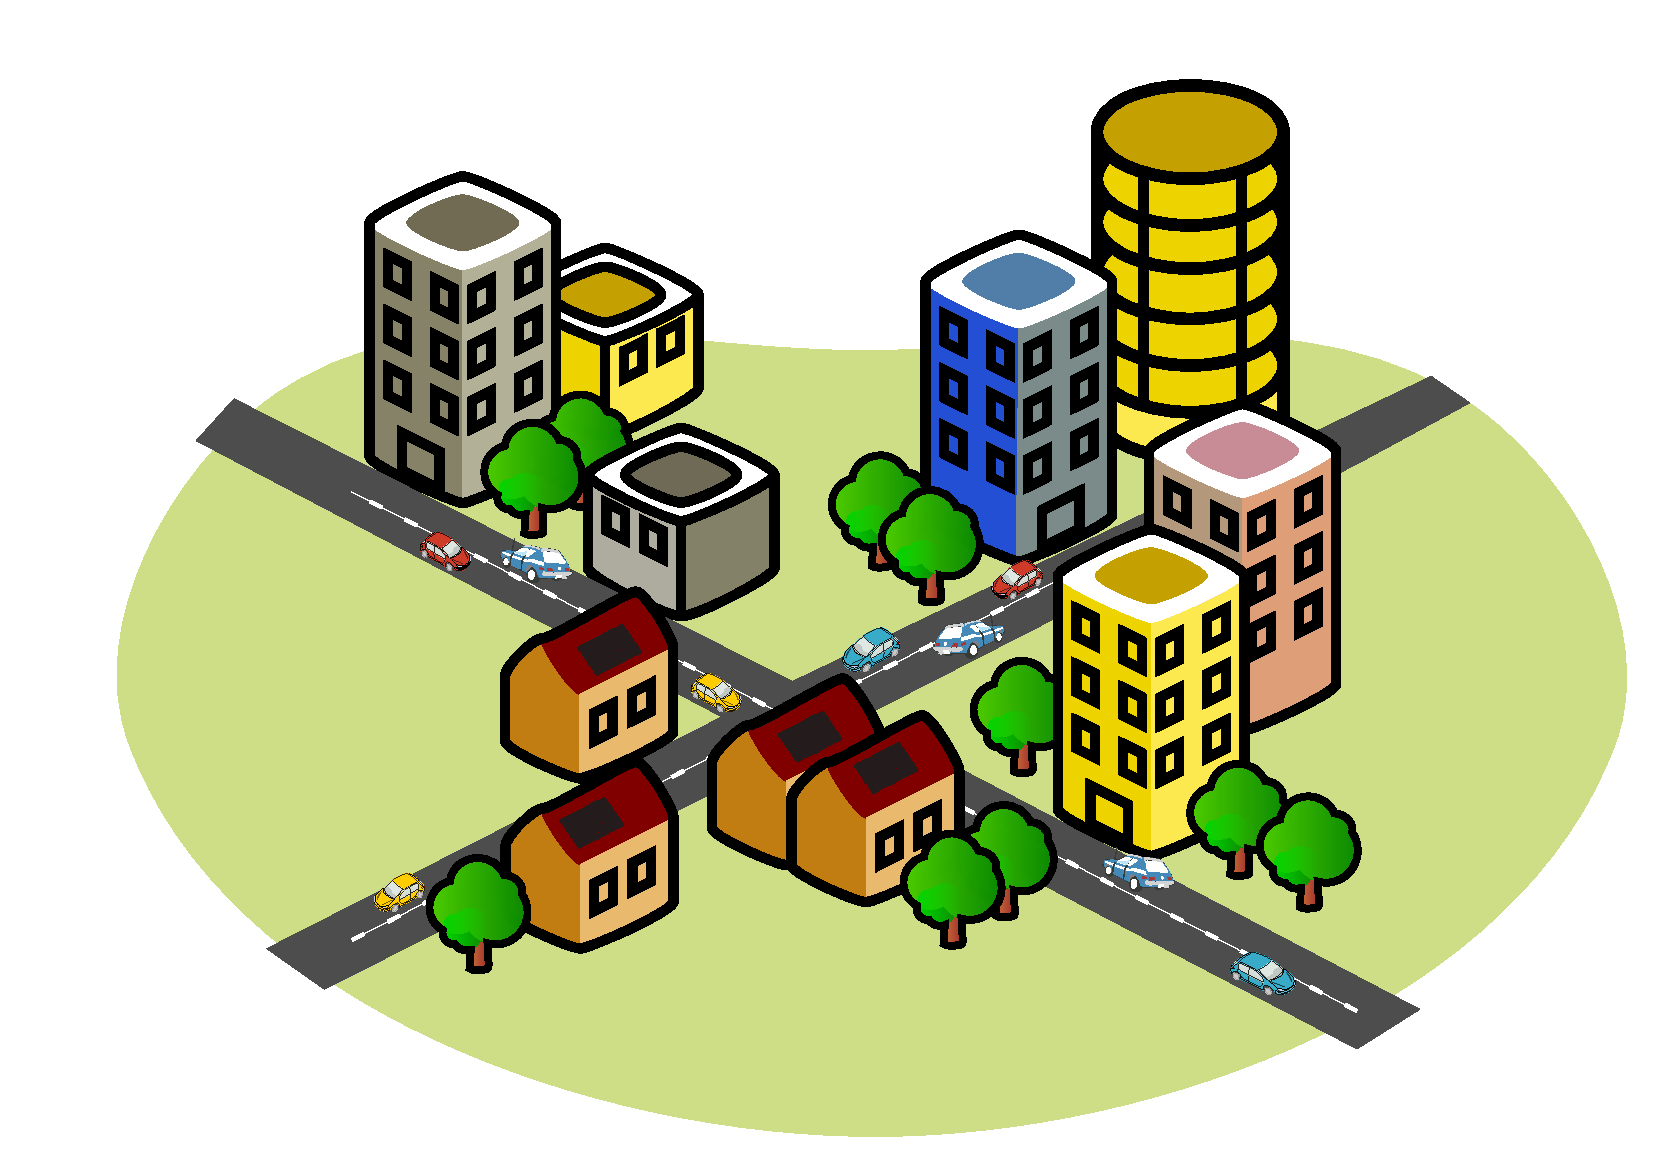
\includegraphics[width=\textwidth]{the_city_cars.pdf}%
%   \end{minipage}
%   \begin{minipage}{.5\textwidth}
%     \begin{itemize}
%       \item<6> Geographically distributed
%       \item<7> Coupled by constraints (energy)
%       \item<8> Optimization objectives
%             \begin{itemize}
%               \item Energy
%               \item User satisfaction
%               \item \dots
%             \end{itemize}
%       \item<9> Solution $\to$ Model Predictive Control
%     \end{itemize}
%   \end{minipage}
%   }
% \end{frame}


% \begin{frame}{Model Predictive Control}
%   Objective: Find control input sequence that optimizes an objective function
%   \only<1-5>{\begin{equation*}
%     \begin{matrix}
%       \underset{\vec{u}(k:k+\alert<3>{N_{p}}-1|k)}{\mathrm{optimize}}&\alert<2>{J(\vec{x}(k),\vec{u}(k))}\\
%       \mathrm{subject~ to}&
%       \left.
%         \begin{matrix}
%           \alert<4>{\vec{x}(\xi+1)=f(\vec{x}(\xi),\vec{u}(\xi))}\\
%           \alert<5>{g_{i}(\vec{x}(\xi),\vec{u}(\xi))\leq0}\\
%           \alert<5>{h_{j}(\vec{x}(\xi),\vec{u}(\xi))=0}\\
%         \end{matrix}
%       \right\}
%       \begin{aligned}
%         &\forall \xi\in\{1,\dots,\alert<3>{N_{p}}\}\\
%         &\forall i\in\{1,\dots,m\}\\
%         &\forall j\in\{1,\dots,p\}
%       \end{aligned}
%     \end{matrix}
%   \end{equation*}}%
% \only<6->{
%   \begin{equation*}
%     \begin{matrix}
%       \underset{\vec{u}(k:k+N_{p}-1|k)}{\mathrm{minimize}}&  \sum_{j=1}^{N_{p}}\|\vec{v}(k+j|k)\|^{2}_{Q}+\|\vec{u}(k+j-1|k)\|^{2}_{R}\\
%       \mathrm{subject~ to}&
%       \left.
%         \begin{matrix}
%           \vec{x}(\xi+1)=f(\vec{x}(\xi),\vec{u}(\xi)) \\
%           g_{i}(\vec{x}(\xi),\vec{u}(\xi))\leq0\\
%           h_{j}(\vec{x}(\xi),\vec{u}(\xi))=0\\
%         \end{matrix}
%       \right\}
%       \begin{aligned}
%         &\forall \xi\in\{1,\dots,N_{p}\}\\
%         &\forall i\in\{1,\dots,m\}\\
%         &\forall j\in\{1,\dots,p\}
%       \end{aligned}
%     \end{matrix}
%   \end{equation*}
%   }%
%   \script<1->{The Model based Predictive Control, for those who don't know is a control strategy where the control is computed by solving an optimization problem }
%   \script<2->{with cost J. }
%   \script<3->{The system's response for the input u is predicted for a period Np, }
%   \script<4->{using the model of the system. }
%   \script<5->{And we then add the equality and inequality constraints. }
%   \script<6->{Usually the optimization problem is to minimize a quadratic objective function.}
% \end{frame}

\newlength\fheight
\newlength\fwidth
\setlength\fwidth{.35\textwidth}
\setlength\fheight{.8\fwidth}

\begin{frame}{Model Predictive Control}{In a nutshell}
  \small
  \begin{overlayarea}{\textwidth}{\textwidth}
  \onslide<2->{Find optimal control sequence}%
  \only<3->{, apply first element}%
  \only<4->{, rinse repeat}%
  \only<5->{ $\to$ Receding Horizon}%

  \begin{figure}
    \centering
    \foreach \i in {1,...,6}{%
      % \includegraphics<\i>[width=.5\textwidth]{mpc\i.pdf}%
      \only<{\i}>{\input{../img/mpcState\i.tex}}%
      \only<{\i}>{\input{../img/mpcControl\i.tex}}%
    }
  \end{figure}
  \end{overlayarea}
  \script<1->{We find an optimal control sequence }
  \script<2->{We apply only the first element }
  \script<3->{and then we repeat }
\end{frame}

\begin{frame}{Distributed Model Predictive Control}
  \begin{itemize}
    \item<1> Problem: Complexity depends on $\predhorz,m,p$ and sizes of $\vec{x}$ and $\vec{u}$
    \item<2-> Solution: Divide and Conquer\footnote{\footnotesize\visible<2->{\lower4pt\hbox{\pgfuseimage{beamericonbook}} \citetitle{MaestreEtAl2014}}}
  \end{itemize}
  \vfill
  \centering
  \begin{minipage}[c]{.45\linewidth}
    \begin{figure}
      \centering
      \only<1,2>{
        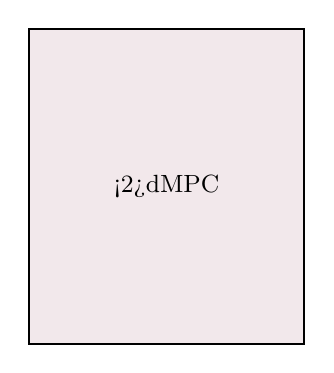
\begin{tikzpicture}[font=\small,thick,node distance=.6cm and 6cm]
          \node[draw,
          rectangle,
          trapezium stretches,
          align=center,
          fill=supelecRed!10,
          alt=<{1}>{fill=supelecRed!90,text=white},
          minimum width=3.5cm,
          minimum height=4cm
          ] (block1) {\only<2>{d}MPC};
        \end{tikzpicture}
      }%
      \only<3->{
        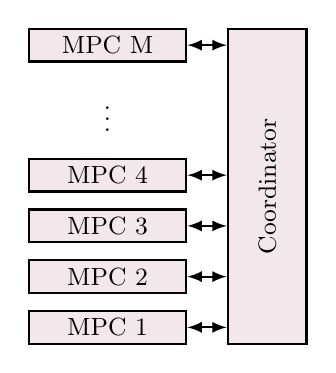
\begin{tikzpicture}[font=\small,thick,node distance=.2cm and 2cm,
          mpcSmall/.style={
            draw,
            rectangle,
            align=center,
            fill=supelecRed!10,
            minimum width=2.cm,
            minimum height=.4cm,
          inner sep=.1cm},
          coordinator/.style={
            draw,
            rectangle,
            align=center,
            fill=supelecRed!10,
            minimum width=1cm,
            minimum height=4cm
          } ]

          \node[mpcSmall] (blockM) {MPC M};

          \node[coordinator, anchor= north west] (coordinator) at ($(blockM.north east) + (.5,0)$) {\rotatebox{90}{Coordinator}};

          \node[ mpcSmall, anchor=south east] (block1) at ($(coordinator.south west) + (-.5,0)$) {MPC 1};
          \node[mpcSmall, above=of block1] (block2) {MPC 2};
          \node[mpcSmall, above=of block2] (block3) {MPC 3};
          \node[mpcSmall, above=of block3] (block4) {MPC 4};
          \node[above=.2cm of block4] (ellips) {\vdots};

          \draw[latex-latex] (block1.east) -- (block1.east -| coordinator.west);
          \draw[latex-latex] (block2.east) -- (block2.east -| coordinator.west);
          \draw[latex-latex] (block3.east) -- (block3.east -| coordinator.west);
          \draw[latex-latex] (block4.east) -- (block4.east -| coordinator.west);
          \draw[latex-latex] (blockM.east) -- (blockM.east -| coordinator.west);
        \end{tikzpicture}
      }%
    \end{figure}
  \end{minipage}
  \script<1->{The problem is when the systems are large, since the complexity depends on Np the number of constraints and sizes of input and states }
  \script<2->{The solution is to divide the problem where it is separable and use a coordinator to create a consensus in the coupling variables or constraints}
\end{frame}

\definecolor{mpc_agent}{RGB}{243, 146, 0} % logo necsys
\colorlet{mpc_agent}{supelecRed!90}
\definecolor{mpc_coordinator}{RGB}{235, 235, 235}
\colorlet{mpc_coordinator}{supelecRed!10}

\newcommand{\tikzmark}[1]{\tikz[baseline={(#1.base)},overlay,remember picture] \node[outer sep=0pt, inner sep=0pt] (#1) {\phantom{A}};}
\begin{frame}{Distributed Model Predictive Control}{Optimization Frameworks}
\begin{minipage}[c]{.45\linewidth}
  \begin{figure}[H]
  \centering
  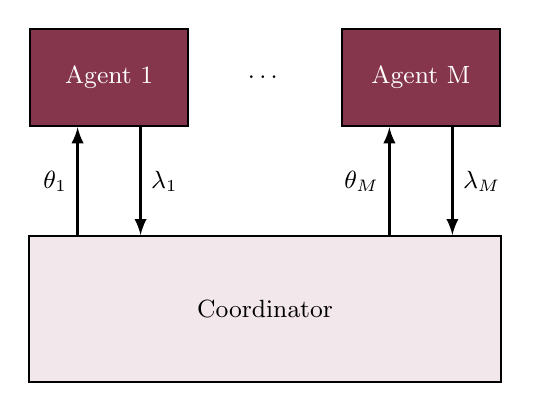
\begin{tikzpicture}[font=\small,thick,node distance=3*0.6180cm and 0.6180cm,every node/.style=rectangle,
    mpcSmall/.style={fill=mpc_agent, minimum height=0.6180*2cm, minimum width=2cm,text=white},
    coordinator/.style={fill=mpc_coordinator, minimum height=0.6180*3cm, minimum width=6cm},
    ]

    \node[draw, mpcSmall] (block1) {\small Agent 1};
    \node[fill=none, draw=none, right=of block1,] (mult) {\bf $\dots$};
    \node[draw, mpcSmall, fill=mpc_agent, right=of mult,] (blockM) {\small Agent M};
    \node[draw, coordinator, below=of mult,] (coordinator) {Coordinator};

    \draw[-latex,line width=1pt] (block1.south)+(0.4,.0) -- ( coordinator.north -| {$(block1.south)+(0.4,.0)$}) node [right,midway] {$\lambda_{1}$};
    \draw[latex-,line width=1pt] (block1.south)+(-0.4,0) -- (  coordinator.north -| {$(block1.south)+(-0.4,0)$}) node [left,midway] {$\theta_{1}$};
    \draw[-latex,line width=1pt] (blockM.south)+(0.4,.0) -- ( coordinator.north -| {$(blockM.south)+(0.4,.0)$}) node [right,midway] {$\lambda_{M}$};
    \draw[latex-,line width=1pt] (blockM.south)+(-0.4,0) -- (  coordinator.north -| {$(blockM.south)+(-0.4,0)$}) node [left,midway] {$\theta_{M}$};
  \end{tikzpicture}
\end{figure}
\end{minipage}
\hfill
\begin{minipage}[c]{.5\linewidth}
  \begin{itemize}
    \item<1-> Agents solve local problems\tikzmark{a}
    \item<2-> Variables are updated
  \end{itemize}
  \onslide<3>{
  \begin{tikzpicture}[overlay, remember picture,decoration={brace,amplitude=2pt}]
    \draw[decorate,thick] (a.north east) --+ (0,-1) node[midway, right=0.1cm,text=black,text width = 2in] {Until\\ Convergence};
  \end{tikzpicture}%
  }
  \centering
\end{minipage}
\end{frame}

\begin{frame}{Distributed Model Predictive Control}
  Negotiation works fine if agents comply.\\\pause
  But what if some agents are ill-intentioned and attack the system?\\~\\\pause
  \begin{itemize}
    \item What are the consequences of an attack?\pause
    \item Can we mitigate the effects?
  \end{itemize}
\end{frame}

\begin{frame}{State of art}{}
  \begin{table}[H]
  \resizebox{1.\textwidth}{!}{
  \begin{tabular}[h]{lccccc}
    \toprule
     & Decomposition & Present vulnerabilities?  & Resilient/Robust & Detection & Mitigation\\
    \midrule
    \alert<2>{\cite{VelardeEtAl2017a}}\\ \cite{MaestreEtAl2021} & Dual & Yes & Robust (Scenario) & NA & NA\\\\
    \cite{VelardeEtAl2017b} \\ \cite{VelardeEtAl2018} & Dual & Yes & Robust (f-robust) & NA & NA\\\\
    \alert<2>{\cite{ChanfreutEtAl2018}} & Jacobi-Gauß & Yes & -- & -- & --\\\\
    \cite{AnandutaEtAl2018}\\\cite{AnandutaEtAl2019}\\\cite{AnandutaEtAl2020} & Dual & Yes & Resilient& Analyt./Learn. & Disconnect (Robustness)\\\\
    \midrule
    Our & Primal & Yes & Resilient & Active Analyt./Learn. & Data reconstruction\\
    \bottomrule
  \end{tabular}
}
\end{table}
\end{frame}


% % Structuring a talk is a difficult task and the following structure
% % may not be suitable. Here are some rules that apply for this
% % solution:

% % - Exactly two or three sections (other than the summary).
% % - At *most* three subsections per section.
% % - Talk about 30s to 2min per frame. So there should be between about
% %   15 and 30 frames, all told.

% % - A conference audience is likely to know very little of what you
% %   are going to talk about. So *simplify*!
% % - In a 20min talk, getting the main ideas across is hard
% %   enough. Leave out details, even if it means being less precise than
% %   you think necessary.
% % - If you omit details that are vital to the proof/implementation,
% %   just say so once. Everybody will be happy with that.

\begin{frame}{Outline}
  % \tableofcontents
  \tableofcontents[subsectionstyle=hide/hide/hide,pausesections]
  % You might wish to add the option [pausesections]
  \script<1->{To respond this this presentation is divided into 3 parts.}
  \script<1->{First We present the vulnerabilites of this decomposition method, }
  \script<2->{We propose one way to secure the method,}
  \script<3->{and finally we present our results.}
\end{frame}

\section[Vulnerabilities in dMPC based on Primal decomposition]{Vulnerabilities in distributed MPC based on Primal Decomposition}

\subsection{What is the Primal Decomposition?}

\begin{frame}{Distributed Model Predictive Control}{Primal Decomposition | Quantity Decomposition | Resource Allocation}
  \vspace{1cm}
  \begin{overlayarea}{\textwidth}{.5\textwidth}
    Decompose \structure<2-3>{original problem} using primal problem
    \only<2>{
      \begin{equation*}
        \begin{matrix}
          \minimize\limits_{\vec{u}[0:\predhorz-1|k]} & J(\vec{x}[0|k],\vec{u}[0:\predhorz-1|k])&\\
          \mathrm{subject~ to} &
                                 \left.
                                 \begin{matrix}
                                   \vec{x}[\xi|k]=f(\vec{x}[\xi-1|k],\vec{u}[\xi-1|k])\\
                                   g_{i}(\vec{x}[\xi-1|k],\vec{u}[\xi-1|k])\leq0\\
                                   h_{j}(\vec{x}[\xi-1|k],\vec{u}[\xi-1|k])=0\\
                                 \end{matrix}
          \right\}
          \begin{aligned}
            &\forall \xi\in\{1,\dots,\alert<5>{\predhorz}\}\\
            &\forall i\in\{1,\dots,m\}\\
            &\forall j\in\{1,\dots,p\}
          \end{aligned}
        \end{matrix}
      \end{equation*}
    }
    \only<3-4>{
      \begin{equation*}
        \begin{matrix}
          \minimize\limits_{\vec{u}[0:\predhorz-1|k]} &\sum\limits_{i\in\set{M}} \sum\limits_{j\in\set{N}}\left[\norm{\tikzmark{a}\alert<4>{\vec{v}_i[j|k]}}^{2}_{Q_i}+\norm{\vec{u}_i[j-1|k]}^{2}_{R_i}\right]&\\
          \mathrm{subject~ to} &
                                 \left.
                                 \begin{matrix}
                                   \vec{x}[\xi|k]=f(\vec{x}[\xi-1|k],\vec{u}[\xi-1|k])\\
                                   g_{i}(\vec{x}[\xi-1|k],\vec{u}[\xi-1|k])\leq0\\
                                   h_{j}(\vec{x}[\xi-1|k],\vec{u}[\xi-1|k])=0\\
                                 \end{matrix}
          \right\}
          \begin{aligned}
            &\forall \xi\in\{1,\dots,\predhorz\}\\
            &\forall i\in\{1,\dots,m\}\\
            &\forall j\in\{1,\dots,p\}
          \end{aligned}
        \end{matrix}
      \end{equation*}
    }
    \only<5>{
      \begin{equation*}
        \begin{matrix}
          \minimize\limits_{\vec{u}[0:\predhorz-1|k]} &\sum\limits_{i\in\set{M}} \sum\limits_{j\in\set{N}}\left[\norm{\tikzmark{a}\vec{v}_i[j|k]}^{2}_{Q_i}+\norm{\vec{u}_i[j-1|k]}^{2}_{R_i}\right]&\\
          \mathrm{subject~ to} &
                                 \left.
                                 \begin{matrix}
                                   \vec{x}[\xi|k]=A\vec{x}[\xi-1|k]+B\vec{u}[\xi-1|k]\\
                                   g_{i}(\vec{x}[\xi-1|k],\vec{u}[\xi-1|k])\leq0\\
                                   h_{j}(\vec{x}[\xi-1|k],\vec{u}[\xi-1|k])=0
                                 \end{matrix}
          \right\}
          \begin{aligned}
            &\forall \xi\in\{1,\dots,\predhorz\}\\
            &\forall i\in\{1,\dots,m\}\\
            &\forall j\in\{1,\dots,p\}
          \end{aligned}
        \end{matrix}
      \end{equation*}
    }
    \only<6>{
      \begin{equation*}
        \begin{matrix}
          \minimize\limits_{\vec{u}[0:\predhorz-1|k]} &\sum\limits_{i\in\set{M}} \sum\limits_{j\in\set{N}}\left[\norm{\tikzmark{a}\vec{v}_i[j|k]}^{2}_{Q_i}+\norm{\vec{u}_i[j-1|k]}^{2}_{R_i}\right]&\\
          \mathrm{subject~ to} &
                                 \left.
                                 \begin{matrix}
                                   \vec{x}[j|k]=A_{i}\vec{x}[j-1|k]+B_{i}\vec{u}[j-1|k]\\
                                   \sum\limits_{i\in\set{M}}\Gamma_{i}\vec{u}_{i}[j|k]\leq\vec{u}_{\mathrm{\max}}
                                 \end{matrix}
          \right\}
          \begin{aligned}
            &\forall j\in\set{N}\\
          \end{aligned}
        \end{matrix}
      \end{equation*}
    }

    \only<4-5>{
      \begin{tikzpicture}[overlay, remember picture]
        \draw[latex-,thick] (a) .. controls +(.5,.5) and +(-0.5,-1.0) .. +(3.5,1) node[above=.25cm,align=center,anchor=center,text=black,text width = 2in] {E.g. ${v_{i}=w_{i}-x_{i}}$};
      \end{tikzpicture}%
    }

    % \only<4>{
    % \begin{equation*}
    %   \scalebox{1}{
    %   $\displaystyle
    %   \begin{matrix}
    %     \minimize\limits_{\vec{u}_i[0:\predhorz-1|k]}&\overbrace{\sum\limits^{M}_{i=1} \overbrace{\sum_{j=1}^{N_{p}}\|\vec{v}_i[j|k]\|^{2}_{Q_i}+\|\vec{u}_i(k+j-1|k)\|^{2}_{R_i}}^{\textstyle J_{i}(k)}}^{\textstyle J_{G}(k)}\\
    %     \mathrm{subject~ to}&
    %     \left.
    %       \begin{matrix}
    %         \vec{x}_{i}(k+1)=A_{i}\vec{x}_{i}(k) + B_{i}\vec{u}_{i}(k)\\
    %         \sum^{M}_{i=1}\Gamma_{i}\vec{u}_{i}(k)=\vec{u}_{\mathrm{\max}}\\
    %       \end{matrix}
    %     \right\}
    %     \begin{aligned}
    %       &\forall i\in\{1,\dots,M\}\\
    %       &\forall j\in\{1,\dots,N_{p}\}
    %     \end{aligned}
    %   \end{matrix}
    %   $}
    % \end{equation*}
    % }
    %   \only<4>{
    %   \begin{equation*}
    %     \scalebox{.8}{
    %     $\displaystyle
    %     \left.
    %       \small
    %       \begin{aligned}
    %         J_{i}^{\star}(\vec{\theta}_{i}(k))&=\underset{\vec{u}_{i}(k:k+N_{p}-1|k)}{\mathrm{minimize}}J_i(k)\\
    %         \mathrm{s.t.} &\quad\vec{x}_{i}(k+1)=A_{i}\vec{x}_{i}(k) + B_{i}\vec{u}_{i}(k)\\
    %         &\quad\Gamma_{i}\vec{u}_i(k)=\vec{\theta}_{i}(k):\vec{\lambda}_{i}(k)\\
    %       \end{aligned}
    %     \right\}
    %     \small
    %     \begin{aligned}
    %       &\forall i\in\{1,\dots,M\}\\
    %       &\forall j\in\{1,\dots,N_{p}\}
    %     \end{aligned}
    %     \label{eq:DOP_local}
    %     $}
    %   \end{equation*}
    %   \vfill
    %   \begin{equation*}
    %     \small
    %     \begin{aligned}
    %       \only<2>{
    %       J^{\star}&=\underset{\vec{\theta}(k:k+N_{p}-1|k)}{\mathrm{minimize}}\sum^{M}_{i=1} J^{\star}_i(\vec{\theta}_i(k))\\
    %       \mathrm{s.t.} &\quad \sum_{i=1}^{M}\vec{\theta}_{i}(k)=\vec{u}_{\max}
    %     }
    %       \only<3->{
    %       \vec{\theta}_{i}\pplusone=\vec{\theta}_{i}\p+\rho\left(\vec{\lambda}_{i}^{\star}(\vec{\theta}_{i}\p)-\frac{1}{M}\sum^{M}_{j=1} \vec{\lambda}_{j}^{\star}(\vec{\theta}_{j}\p)\right)
    %     }
    %     \end{aligned}
    %   \end{equation*}
    % }
  \end{overlayarea}
  \vfill
  \script<1->{An example of decomposition method is the Quantity decomposition where a semi-decomposable problem with a global coupling constraints can be decomposed into }
  \script<2->{multiple sub-problems, which can be solved in parallel, and a master problem which corresponds to the initial problem. \\ Those coupling constraints are replaced by local constraints with an allocation theta i. }
  \script<3->{The allocation for each sub-problem is updated by a projected subgradient method solving the master problem, thus the original problem. The subgradient used in this method is the dual variable associated to the coupling constraints}
  \script<4->{We can represent the sub-problems as agents and the master problem as a coordinator. The coordinator sends the allocations for each agent, which responds with a dual variable. }
\end{frame}
% \begin{frame}
%   \centering
%   \begin{minipage}{.65\linewidth}
%     \begin{algorithm}[H]
%       \DontPrintSemicolon
%       Coordinator initializes $\vec{\theta}^{(0)}$ \;
%       $p:=0$\;
%       \Repeat{$\|\vec{\theta}^{(p)} -\vec{\theta}^{(p-1)}\|\leq\epsilon$}{
%         Subsystems solve~\eqref{eq:DOP_local}, and send $\vec{\lambda}^{\star}_{i}(\vec{\theta}\p)$\;
%         Coordinator updates allocations~\eqref{eq:thetaNegot}\;
%         $p:=p+1$
%       }
%       \caption{Quantity decomposition based DMPC.}\label{alg:quantityAlg}
%     \end{algorithm}
%   \end{minipage}
% \end{frame}

\begin{frame}{Quantity Decomposition | Resource Allocation}
  \centering
  \begin{minipage}{.45\linewidth}
    \begin{figure}
      \centering
      \scalebox{.55}{
        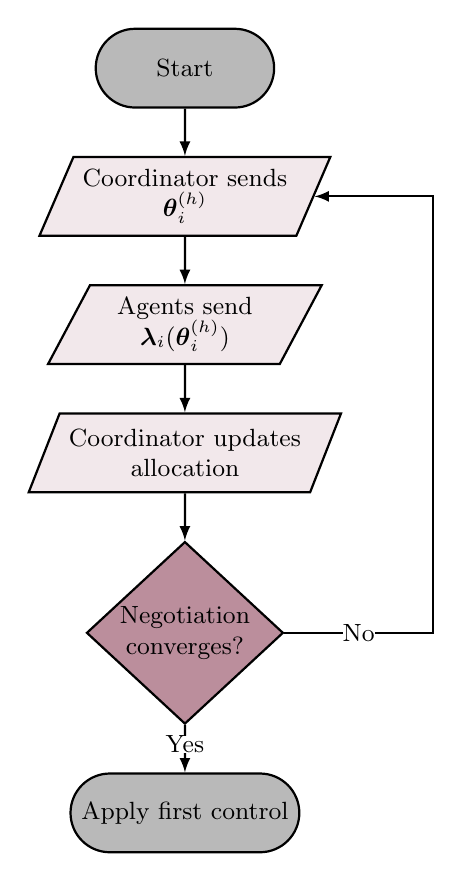
\begin{tikzpicture}[font=\small,thick,node distance=.6cm and 6cm]
          \node[draw,
          rounded rectangle,
          fill=gray!90!black!50,
          alt=<{2}>{fill=supelecRed!90,text=white},
          minimum width=2.5cm,
          minimum height=1cm] (block1) {Start};

          \node[draw,
          trapezium,
          trapezium left angle = 65,
          trapezium right angle = 115,
          trapezium stretches,
          align=center,
          below=of block1,
          fill=supelecRed!10,
          alt=<{3}>{fill=supelecRed!90,text=white},
          minimum width=3.5cm,
          minimum height=1cm
          ] (block7) { Coordinator sends \\$\vec{\theta}_i^{(h)}$};
          \node[draw,
          trapezium,
          trapezium left angle = 65,
          trapezium right angle = 115,
          trapezium stretches,
          align=center,
          fill=supelecRed!10,
          alt=<{4}>{fill=supelecRed!90,text=white},
          below=of block7,
          minimum width=3.5cm,
          minimum height=1cm
          ] (block8) { Agents send \\$\vec{\lambda}_i(\vec{\theta}_{i}^{(h)})$};

          \node[draw,
          trapezium,
          trapezium left angle = 65,
          trapezium right angle = 115,
          trapezium stretches,
          align=center,
          fill=supelecRed!10,
          alt=<{5}>{fill=supelecRed!90,text=white},
          below=of block8,
          minimum width=3.5cm,
          minimum height=1cm
          ] (block9) { Coordinator updates \\allocation};

          \node[draw,
          diamond,
          below=of block9,
          minimum width=2.5cm,
          fill=supelecRed!50,
          alt=<{6}>{fill=supelecRed!90,text=white},
          align=center,
          inner sep=0] (block10) { Negotiation\\ converges?};

          \node[draw,
          rounded rectangle,
          below=of block10,
          fill=gray!90!black!50,
          alt=<{7}>{fill=supelecRed!90,text=white},
          minimum width=2.5cm,
          minimum height=1cm,] (block11) { Apply first control};

          \draw[-latex] (block7) edge (block8)
          (block1) edge (block7)
          (block8) edge (block9)
          (block9) edge (block10);

          \draw[-latex] (block10) -- (block11)
          node[pos=0.4,fill=white,inner sep=0]{Yes};

          \draw[-latex] (block10) -| ($(block7.east) + (1.5cm,0)$)
          node[pos=0.25,fill=white,inner sep=0]{No} -- (block7.east);

        \end{tikzpicture}
      }
      % \caption{Quantity decomposition based DMPC}\label{fig:quantityDecompDMPC}
    \end{figure}
  \end{minipage}
  \only<7->{\begin{minipage}{.45\linewidth}
    \begin{figure}
      \centering
      % \includegraphics[width=\textwidth]{dmpcQuantity4systemsTriche_.mat_thetalambdanegot.pdf}
    \end{figure}
  \end{minipage}}
  \script<1->{In a flowchart for a quantity decomposition based DMPC,}
  \script<3->{the coordinator sends the allocation theta, }
  \script<4->{the agents send the dual variable lambda, }
  \script<5->{the coordinator updates the allocation. }
  \script<6->{If negotiation converges, }
  \script<7->{then the negotiation ends and each agent applies the first element of the control found}
\end{frame}

% \begin{frame}{}
%   \centering
%   \vfill
% What if agents send a non-agreed $\vec{\lambda}_{i}$?
%   \vfill
%   \script<1>{But what if the agents send a non-agreed lambda?}
% \end{frame}


\subsection{How can an agent attack?}

\begin{frame}{How can a non-cooperative agent attack?}

  \begin{itemize}
    \item<1-> $\vec{\lambda}_{i}$ is the only interface with coordination
    \item<2-> Non-cooperative agent sends $\tilde{\vec{\lambda}}_{i}=\gamma_{i}(\vec{\lambda}_{i})$\pause
  \end{itemize}
\script<1->{How can an agent attack the system? Its only interface with the coordination is lambda}
\script<2->{so we suppose it attacks by sending a different $lambda_i$, modified by a function $gamma_i$ of $lambda_i$ }
\end{frame}

\subsection{Consequences}
% \begin{frame}{Example}
%   \begin{minipage}[c]{.45\linewidth}
%     \begin{figure}[!t]
%       \centering
%       \begin{tikzpicture}
%         % \node (0,0){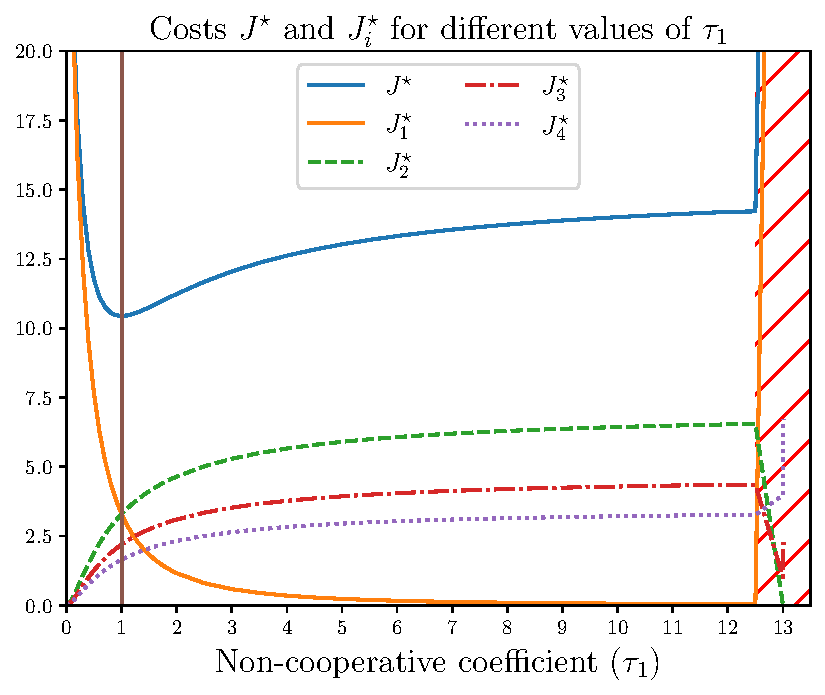
\includegraphics[width=\textwidth]{changeOfJ.pdf}};
%         \draw<4>[rounded corners,red,thick] (-2.3,2.5) rectangle +(.5,-5);
%         \draw<5>[rounded corners,red,thick] (2.3,2.5) rectangle +(.75,-5);
%       \end{tikzpicture}
%     \end{figure}
%   \end{minipage}
%   \hfill
%   \begin{minipage}[c]{.45\linewidth}
%     \begin{exampleblock}{4 distinct agents}
%       \begin{itemize}
%         \item<2-> Agent 1 is non-cooperative\\
%         \item<3-> It uses $\tilde{\vec{\lambda}}_{1}=\gamma_{1}(\vec{\lambda}_{1})=\tau_{1}I\vec{\lambda}_{1}$
%       \end{itemize}
%     \end{exampleblock}
%   \end{minipage}
% \script<1->{We give an example of 4 agents negotiating }
% \script<2->{Agent 1 is non-cooperative\\ }
% \script<3->{It uses a linear cheating function gamma tau times identity times the original lambda i\\ }
% \script<3->{In the figure we can see the cost functions for each agent, we see that agent 1 cost decreases if we increase tau, but the overall cost is increased, The minimum value of the global cost is when \\ }
% \script<4->{tau is equal to one. If tau is close to zero it increases its cost and if tau is too high\\ }
% \script<5->{it can turn the negotiation unstable \\ }
% \end{frame}

% \section{Securing the DMPC}
% \script<1->{In order to secure the method let's analyze the subproblems \\ }

% \subsection{Analysis of Subproblems}

% \begin{frame}
%   \frametitle{Quadratic Case}
%   \only<1>{
%     \begin{equation*}
%       % \scalebox{.8}{
%       %   $\displaystyle
%           \small
%           \begin{aligned}
%             \underset{\vec{u}_{i}(k:k+N_{p}-1|k)}{\mathrm{minimize}}&\overbrace{\sum_{j=1}^{N_{p}}\|\vec{v}_i(k+j|k)\|^{2}_{Q_i}+\|\vec{u}_i(k+j-1|k)\|^{2}_{R_i}}^{\textstyle J_{i}(k)}\\
%             \mathrm{s.t.} &
%             \left.
%               \begin{aligned}
%                 \vec{x}_{i}(\xi+1)=A_{i}\vec{x}_{i}(\xi) + B_{i}\vec{u}_{i}(\xi)\\
%                 \Gamma_{i}\vec{u}_i(\xi)=\vec{\theta}_{i}(\xi):\vec{\lambda}_{i}(\xi)\\
%               \end{aligned}
%             \right\}
%             \small
%             \begin{aligned}
%               &\forall \xi\in\{1,\dots,N_{p}\}
%             \end{aligned}
%           \end{aligned}
%           \label{eq:DOP_local}
%         % $}
%     \end{equation*}

%   }
%   \only<2->{\begin{equation*}
%     \begin{matrix}
%       \underset{\vec{U}_i(k)}{\mathrm{minimize}}& \overbrace{\frac{1}{2}{\vec{U}_i(k)}^T \alert<3>{H_i}\vec{U}_i(k)+{\alert<4>{\vec{f}_i(k)}}^T\vec{U}_i(k)}^{\textstyle J_{i}(\vec{\theta}_{i})}\\
%       \mathrm{s.t.}&\Theta_{i}\vec{U}_i(k)=\vec{\theta}_{i}:\alert<5>{\vec{\lambda}_{i}}\\
%     \end{matrix}
%   \end{equation*}
%   }
%   \only<6->{
%     \begin{equation*}
%       \vec{\lambda}_{i}=-\alert<7>{P_{i}}\vec{\theta}_{i}-\alert<8>{\vec{s}_{i}(k)}
%     \end{equation*}
%     \centering
%     where ${\alert<7>{P_{i}}={(\Theta_{i}H_{i}^{-1}\Theta_{i}\T)}^{-1}}$ and ${\alert<8>{\vec{s}_{i}(k)}=P_{i}\Theta_{i}H_{i}^{-1}\vec{f}_{i}(k)}$
%   }
% \script<1->{If we have a linear system with a quadratic objective function as in the reference tracking problem where we want to minimize the tracking error and the input power\\ }
% \script<2->{we can rewrite as a quadratic program\\ }
% \script<3->{with parameters H\\ }
% \script<4->{and f \\ }
% \script<5->{If we have equality constraints, the dual variables can be calculated explicitly\\ }
% \script<6->{it is an affine function with parameters P and s\\ }
% \script<7->{Observe that P does not depend on the time k\\ }
% \script<8->{meanwhile s does depend, we can use these facts for the detection and mitigation mechanisms\\ }
% \end{frame}

% \subsection{Detection Mechanism}
% \begin{frame}{Detection}
% \begin{assumption}
%   We know nominal $\bar{P}_{i}$
% \end{assumption}
% \pause
% \begin{assumption}
%   Attacker chooses $\tilde{\vec{\lambda}_{i}}=\gamma_{i}(\vec{\lambda}_{i})=T_{i}(k)\vec{\lambda}_{i} $


%  \pause $-T_{i}(k)P_{i}\vec{\theta}_{i}-T_{i}(k)\vec{s}_{i}(k)$ $\to$ $-\tilde{P}_{i}\vec{\theta}_{i}-\tilde{\vec{s}_{i}}(k)$
% \end{assumption}
% \pause
% \begin{itemize}
%   \item We can estimate%
%         \footnote[1]{Using Recursive Least Squares}
%         $\hat{P}_{i}$ and $\widehat{\tilde{\vec{s}}}_{i}(k)$ such as:
%         \begin{equation*}
%           \label{eq:lambdafuntheta_tilde}
%           \tilde{\vec{\lambda}_{i}}=\gamma_{i}(\vec{\lambda}_{i}(\vec{\theta}_{i}))=-\widehat{\tilde{P}_{i}}(k)\vec{\theta}_{i}-\widehat{\tilde{\vec{s}}}_{i}(k)
%         \end{equation*}
% \pause
% \item If $\widehat{\tilde{{P}}}_{i}(k)\neq\bar{{P}}_{i}$ $\to$ Attack
% \end{itemize}
% \script<1->{For the attack detection, let's assume we know the nominal P, called P bar \\ }
% \script<2->{And we also assume the attacker chooses a linear attack where the lambda sent is equal to a matrix T times the original lambda which yields the formula shown \\ }
% \script<3->{with modified P and s, called P tilde and s tilde\\ }
% \script<4->{Now we can estimate P tilde and s tilde for a given negotiation in time k\\ }
% \script<5->{and if the estimated P tilde is different from the nominal P, then there is an attack\\ }

% \end{frame}

% \begin{frame}{About Estimation}
%   \centering
%   \begin{itemize}
%     \item We estimate $\hat{P}_{i}$ and $\widehat{\tilde{\vec{s}}}_{i}(k)$ simultaneously using Recursive Least Squares
%           \pause
%     \item Problem: Estimation during negotiation fails
%           \pause
%           \begin{itemize}
%             \item Consecutive $\vec{\lambda}_{i}^{p}$ and $\vec{\theta}_{i}^{p}$ are linearly dependent $\to$ low input excitation
%           \end{itemize}
%           \pause
%     \item Solution: Send sequence of random values of $\vec{\theta}_{i}$ until estimates converge
%   \end{itemize}
% \script<1->{In order to estimate the modified P and s, we use recursive least squares\\ }
% \script<2->{The problem of estimating the value during a normal negotiation is that it fails\\ }
% \script<3->{Consecutive lambdas and thetas are linearly dependent, since they are calculate via the projected subgradient method, which gives us low input excitation\\ }
% \script<4->{In order to increase the input excitation we send a sequence of random theta until the convergence is attained\\ }
% \end{frame}

% \begin{frame}{Detection}{In detail}
%   \pause
%   \begin{itemize}
%     \item Error ${E_{i}(k) =\|\widehat{\tilde{P}}_{i}(k)-\bar{P}_{i}\|_{F}}$
%           \pause
%     \item Create threshold $\epsilon_{P}$
%           \pause
%     \item Indicator ${d_{i}\in\{0,1\}}$ detects the attack in agent $i$.
%           \pause
%     \item $d_{i}=1$ if $E_{i}(k)>\epsilon_{P}$, $0$ otherwise
%   \end{itemize}
% \script<1->{So, let's detail the detection mechanism.\\ }
% \script<2->{First we calculate the norm of the error between the estimated P and the nominal. (Here we use the Frobenius norm)\\ }
% \script<3->{Then, we create a threshold epsilon p\\ }
% \script<4->{and finally we create an indicator d $i$ for the attack of agent $i$\\ }
% \script<5->{It is equal to 1 if the error is greater than the threshold, indicating an attack or 0 otherwise\\ }
% \end{frame}

% \subsection{Mitigation Mechanism}

% \begin{frame}{Mitigation}
%   \begin{itemize}
%     \item Main idea: Reconstruct $\vec{\lambda}_{i}$ and use in negotiation
%   \end{itemize}
%   \pause
%   \begin{assumption}
%     We suppose ${\tilde{\vec{\lambda}}_{i}=\vec{0}}$ only if ${\vec{\lambda}_{i}=\vec{0}}$, which implies $T_{i}(k)$ invertible.
% \end{assumption}\pause
% \begin{itemize}
%   \item Estimate the inverse of $T_{i}(k)$
%         \begin{equation*}
%           {\widehat{T_{i}(k)^{-1}}=\bar{P}_{i}\widehat{\tilde{P}_{i}}(k)^{-1}}
%         \end{equation*}
%         \pause
%   \item Reconstruct $\vec{\lambda}_{i}$
%         \begin{equation*}
%           {\vec{\lambda}_{i}}_{\mathrm{rec}}=\widehat{T_{i}(k)^{-1}} \tilde{\vec{\lambda}_{i}} =-\bar{P}_{i}\vec{\theta}_{i}-\widehat{{T_{i}(k)^{-1}}}\widehat{\tilde{\vec{s}}}_{i}(k)
%         \end{equation*}

% \end{itemize}
% \script<1->{Now, for the mitigation the main idea is to reconstruct the original lambda from the estimated parameters and use it in the negotiation\\ }
% \script<2->{We suppose the agent wants to decrease its cost, and the lambda sent is only equal to zero if the original is equal to zero. which implies the matrix T is invertible\\ }
% \script<3->{We can estimate the inverse of T, by using the estimate of P tilde and the nominal value of P like in this equation\\ }
% \script<4->{With the estimate of the inverse of T and the estimate of s tilde, we can reconstruct the original lambda\\ }
% \end{frame}

% \subsection{Complete Mechanism}

% \begin{frame}{Complete Mechanism}
%   \begin{minipage}[c]{.45\linewidth}
%     \begin{figure}[b]
%       \centering
%       \scalebox{.7}{\footnotesize \def\svgwidth{12cm}
%       \input{../img/diagQuantSafe2.pdf_tex}}
%       % \caption{Scheme for Secure DMPC}\label{fig:schemeSafeQuantity}
%     \end{figure}
%   \end{minipage}
%   \pause
%   \hfill
%   \begin{minipage}[c]{.45\linewidth}
%     Two phases:
%     \pause
%     \begin{enumerate}
%       \item Detect which agents are non-cooperative
%             \pause
%       \item Reconstruct $\vec{\lambda}_{i}$ and use in negotiation
%     \end{enumerate}
%   \end{minipage}
% \script<1->{The complete mechanism is equivalent to add a supervisor for each agent inside the coordinator\\ }
% \script<2->{The mechanism is divided into the two phases, }
% \script<3->{first we detect which agents are non-cooperative }
% \script<4->{and then reconstruct the lambda i s and use in the usual negotiation\\ }
% \end{frame}

% % \begin{frame}
% % \SetKwBlock{negotPhase}{ Negotiation Phase:}{}
% % \SetKwBlock{detectPhase}{ Detection Phase:}{}
% % \scalebox{.8}{  \begin{algorithm}[H]
% %     \DontPrintSemicolon
% %     \detectPhase{
% %     $h:=0$\;
% %     \Repeat{
% %     $\|\eta_{i}^{h}-\eta^{h-1}\|\leq\epsilon$
% %   }{
% %     Coordinator sets random $\vec{\theta}_{i}^{(h+1)}$ \;
% %     Subsystems solve~\eqref{eq:DOP_local}, and send $\vec{\lambda}^{\star}_{i}(\vec{\theta}^{(h)})$\;
% %     Coordinator estimates $\widehat{\tilde{P}}_{i}(k)^{(h)}$ and $\widehat{\tilde{\vec{s}}}_{i}(k)^{(h)}$ \;
% %     $h:=h+1$\;
% %   }
% %     Coordinator computes $d_{i}$ using~\eqref{eq:2}\;
% %   }
% %     \negotPhase{
% %     Coordinator initializes $\vec{\theta}^{(0)}$ \;
% %     $p:=0$\;

% %     \Repeat{$\|\vec{\theta}^{(p)} -\vec{\theta}^{(p-1)}\|\leq\epsilon$}{
% %     Subsystems solve~\eqref{eq:DOP_local}, and send $\vec{\lambda}^{\star}_{i}(\vec{\theta}\p)$\;

% %     Coordinator updates allocation~\eqref{eq:thetaNegot} using adequate versions of $\vec{\lambda}_{i}$ for each agent: $\vec{\lambda}_{i}^{\star}(\vec{\theta}\p)$, if $d_{i}=0$ and ${\vec{\lambda}_{i}}_{\mathrm{rec}}$, if ${d_{i}=1}$\;
% %     $p:=p+1$
% %   }}
% %     \caption{Secure DMPC.}\label{alg:safeDMPC}
% %   \end{algorithm}
% %   }
% % \end{frame}

% \begin{frame}{Secure DMPC}
%   \begin{figure}[h]
%     \centering
%   \scalebox{.55}{
%     \begin{tikzpicture}[font=\small,thick,node distance=.6cm and 6cm]
%       \draw[loosely dashed,
%       minimum width=2.5cm,
%       minimum height=1cm] (8cm,1cm) -- (8cm,-10cm);

%       \node[] at (5cm,0cm) {\Large \alert<2>{Detection Phase}};
%       \node[] at (11cm,0cm) {\Large \alert<3>{Negotiation Phase}};

%       \node[draw,
%       rounded rectangle,
%       fill=gray!90!black!50,
%       alt=<{4}>{fill=supelecRed!90,text=white},
%       minimum width=2.5cm,
%       minimum height=1cm] (block1) {Start};

%       \node[draw,
%       trapezium,
%       trapezium left angle = 65,
%       trapezium right angle = 115,
%       trapezium stretches,
%       align=center,
%       fill=supelecRed!10,
%       alt=<{5}>{fill=supelecRed!90,text=white},
%       below=of block1,
%       minimum width=3.5cm,
%       minimum height=1cm
%       ] (block2) { Coordinator sends \\random $\vec{\theta}_{i}^{(h)}$};

%       \node[draw,
%       trapezium,
%       trapezium left angle = 65,
%       trapezium right angle = 115,
%       trapezium stretches,
%       align=center,
%       fill=supelecRed!10,
%       alt=<{6}>{fill=supelecRed!90,text=white},
%       below=of block2,
%       minimum width=3.5cm,
%       minimum height=1cm
%       ] (block3) { Agents send \\ $\vec{\lambda}_{i}^{(h)}(\vec{\theta}_{i}^{(h)})$};

%       \node[draw,
%       trapezium,
%       trapezium left angle = 65,
%       trapezium right angle = 115,
%       trapezium stretches,
%       align=center,
%       below=of block3,
%       fill=supelecRed!10,
%       alt=<{7}>{fill=supelecRed!90,text=white},
%       minimum width=3.5cm,
%       minimum height=1cm
%       ] (block4) { Coordinator estimate parameters};

%       \node[draw,
%       diamond,
%       below=of block4,
%       minimum width=2.5cm,
%       fill=supelecRed!50,
%       alt=<{8}>{fill=supelecRed!90,text=white},
%       align=center,
%       inner sep=0] (block5) { Estimates\\ converge?};

%       \node[draw,
%       trapezium,
%       trapezium left angle = 65,
%       trapezium right angle = 115,
%       trapezium stretches,
%       align=center,
%       fill=supelecRed!10,
%       alt=<{9}>{fill=supelecRed!90,text=white},
%       right=1cm of block5,
%       minimum width=3.5cm,
%       minimum height=1cm
%       ] (block6) { Coordinator detects \\selfish agents};

%       \node[coordinate,right=6.cm of block2] (block12) {};

%       \node[draw,
%       trapezium,
%       trapezium left angle = 65,
%       trapezium right angle = 115,
%       trapezium stretches,
%       align=center,
%       right=of block12,
%       fill=supelecRed!10,
%       alt=<{10}>{fill=supelecRed!90,text=white},
%       minimum width=3.5cm,
%       minimum height=1cm
%       ] (block7) { Coordinator sends \\$\vec{\theta}_i^{(h)}$};
%       \node[draw,
%       trapezium,
%       trapezium left angle = 65,
%       trapezium right angle = 115,
%       trapezium stretches,
%       align=center,
%       fill=supelecRed!10,
%       alt=<{11}>{fill=supelecRed!90,text=white},
%       below=of block7,
%       minimum width=3.5cm,
%       minimum height=1cm
%       ] (block8) { Agents send \\$\vec{\lambda}_i(\vec{\theta}_{i}^{(h)})$};

%       \node[draw,
%       trapezium,
%       trapezium left angle = 65,
%       trapezium right angle = 115,
%       trapezium stretches,
%       align=center,
%       fill=supelecRed!10,
%       alt=<{12}>{fill=supelecRed!90,text=white},
%       below=of block8,
%       minimum width=3.5cm,
%       minimum height=1cm
%       ] (block9) { Coordinator updates \\allocation accordingly};

%       \node[draw,
%       diamond,
%       below=of block9,
%       minimum width=2.5cm,
%       fill=supelecRed!50,
%       alt=<{13}>{fill=supelecRed!90,text=white},
%       align=center,
%       inner sep=0] (block10) { Negotiation\\ converges?};

%       \node[draw,
%       rounded rectangle,
%       below=of block10,
%       fill=gray!90!black!50,
%       alt=<{14}>{fill=supelecRed!90,text=white},
%       minimum width=2.5cm,
%       minimum height=1cm,] (block11) { Apply first control};

%       \draw[-latex] (block1) edge (block2)
%       (block2) edge (block3)
%       (block3) edge (block4)
%       (block4) edge (block5);

%       \draw[-latex] (block7) edge (block8)
%       (block8) edge (block9)
%       (block9) edge (block10);

%       \draw[-latex] (block5) -- (block6)
%       node[pos=0.4,fill=white,inner sep=0]{Yes};

%       \draw[-latex] (block10) -- (block11)
%       node[pos=0.4,fill=white,inner sep=0]{Yes};

%       \draw[-latex] (block6) -| ($(block7.west) - (3cm,0)$) -- (block7.west);

%       \draw[-latex] (block10) -| ($(block7.east) + (1.5cm,0)$)
%       node[pos=0.25,fill=white,inner sep=0]{No} -- (block7.east);

%       \draw[-latex] (block5) -| ($(block2.west) - (1.5cm,0)$)
%       node[pos=0.25,fill=white,inner sep=0]{No} -- (block2.west);
%     \end{tikzpicture}
%     }
%     % \caption{Secure DMPC}\label{fig:secureDMPC}
%   \end{figure}
%   \script<1->{Now, for the complete secure DMPC algorithm, as said it is divided into two phases\\ }
%   \script<2->{The Detection phase \\ }
%   \script<3->{and the negotiation phase\\ }
%   \script<5->{The coordinator sends random theta i\\ }
%   \script<6->{The agents send dual variable lambda i\\ }
%   \script<7->{The coordinator estimates the parameters P and s tilde\\ }
%   \script<8->{when the estimates converge\\ }
%   \script<9->{The coordinator detects which agents are non-cooperative\\ }
%   \script<10->{then the negotiation phase begins, the coordinator sends the theta i\\ }
%   \script<11->{the agents send the dual variable lambda i\\ }
%   \script<12->{and the coordinator updates the allocation accordingly using the reconstructed lambda or the one sent by the agent\\ }
%   \script<13->{and once the negotiation converges\\ }
%   \script<14->{each agent applies the first control\\ }

% \end{frame}

% \section{Results}
% \script{Now, for some results}
% \begin{frame}{Example}
%   \begin{exampleblock}{Temperature Control of 4 Distinct Rooms Under Power Scarcity}
%     \begin{itemize}
%             \pause
%       \item 4 distinct rooms modeled using 3R-2C
%             \pause
%       \item Initial temperature under $20^{o}\mathrm{C}$
%             \pause
%       \item Not enough power to achieve setpoint $\left({\sum_{i=1}^{4} \vec{u}_{i}(k)\leq4\mathrm{kW}}\right)$
%             \pause
%       \item Simulated for a period of ${5} \mathrm{h}$
%             \pause
%       \item ZOH ${T_{s}=0.25\mathrm{h}}$
%             \pause
%       \item 3 scenarios
%             \begin{enumerate}
%               \item Nominal
%               \item Agent I non cooperative from k>6 with T=4*I
%               \item Similar but with secure algorithm
%             \end{enumerate}
%     \end{itemize}
%   \end{exampleblock}
%   \script<1->{We give an academic example of the temperature control of 4 distinct rooms under power scarcity\\}
%   \script<2->{The 4 rooms are distinct using the 3 resistor 2 capacitor model\\}
%   \script<3->{the initial temperature of all rooms is under 20 degrees celsius, which is the final setpoint\\}
%   \script<4->{But they are under power scarcity that prevents them from reaching the setpoint\\}
%   \script<5->{we simulate for a period of 5h\\}
%   \script<6->{with sampling time of 15 minutes\\}
%   \script<7->{3 scenarios are simulated, the nominal, one where agent 1 presents non cooperative behavior from k greater than 6, and another with the selfish behavior and the secure mechanism activated\\}
% \end{frame}

% \begin{frame}{Results}{Temporal}
%   \begin{minipage}[c]{.5\linewidth}
%     \begin{figure}[t]
%       \centering
%       %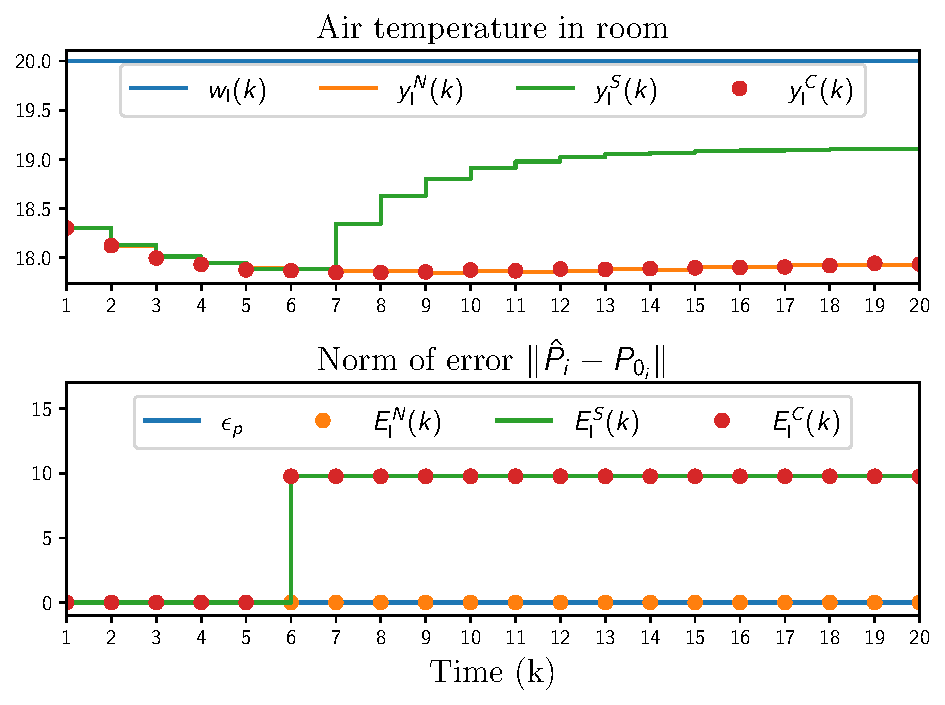
\includegraphics[width=\textwidth]{AirTempAndDecisionVariable.pdf}
%       % \caption{Temperature in room I and the decision variable $E_{I}(k)$}\label{fig:response3Scenarios}
%     \end{figure}
%   \end{minipage}
%   \hfill
%   \begin{minipage}[c]{.45\linewidth}
%     \begin{itemize}
%       \item[N] Nominal
%       \item[S] Selflish behavior
%       \item[C] selfish behavior with Correction
%     \end{itemize}\pause
%   \end{minipage}
%   \script<1->{In the figure we see the air temperature and the estimation error for room 1\\}
%   \script<2->{The nominal behavior is in orange, and as said it cannot reach the setpoint, in blue\\}
%   \script<3->{When the room presents selfish behavior (in blue), it reduces its cost and get closer to the setpoint, we see that the attack increases the error\\}
%   \script<4->{Now, for the case with correction (the red dots), even if it attacks the system, the temperature is close to its nominal value\\}
% \end{frame}

% \begin{frame}
% \frametitle{Results}
%   \begin{table}[t]
%   \centering
%   \caption{Comparison of costs $J_{i}^{N}$ and $J_{G}^{N}$}\label{tab:costsGlobalLocal}
%   \begin{tabular}[t]{cccc} \toprule
%     Agent  & Nominal & Selfish & Selfish + correction\\
%     \midrule
%     I      & 103  &  64  & 104  \\
%     II     &  73  &  91  &  73  \\
%     III    & 100  & 123  & 101  \\
%     IV     & 132  & 154  & 131  \\
%     Global & 408  & 442  & 409  \\
%     \bottomrule
%   \end{tabular}
%   \pause
%   \script<1->{Now, if we compare the costs for each scenario we see how the cost of agent 1 decreases when it attacks, while the cost of other agents increase.\\}
%   \script<2->{When the secure algorithm is activated the costs are very close to the original ones. So }
% \end{table}

% \end{frame}
\section*{Summary}

% \begin{frame}{Summary}
%   \pause
%   \begin{minipage}[t]{.45\textwidth}
%     % Keep the summary *very short*.
%     \begin{enumerate}
%       \item
%             Resource allocation based DMPC is vulnerable to attacks.
%             \pause
%       \item
%             Sub-problems' structure has time invariant parameters.
%             \pause
%       \item Attacks can be detected using these parameters.
%             \pause
%       \item Effects can be mitigated.
%     \end{enumerate}
%   \end{minipage}
%   \pause
%     % The following outlook is optional.
%     % \vskip0pt plus.5fill
%   \begin{minipage}[t]{.45\textwidth}
%     \begin{itemize}
%       \item Outlook
%             \pause
%             \begin{itemize}
%               \item
%                     Inequality Constraints yield Hybrid behavior
%                     \pause
%               \item
%                     Non-linear attack model
%             \end{itemize}
%     \end{itemize}
%   \end{minipage}
%   \script<1->{We can see that\\}
%   \script<2->{Resource allocation based DMPC is vulnerable to attacks.\\}
%   \script<3->{Sub-problems' structure has time invariant parameters.\\}
%   \script<4->{Attacks can be detected using these parameters.\\}
%   \script<5->{and Effects can be mitigated.\\}
%   \script<6->{An outlook for future works \\}
%   \script<7->{is to use inequality constraints instead of only equality constraints, which will yield hybrid behavior\\}
%   \script<8->{and try to implement with non-linear attack models\\}

% \end{frame}



\begin{frame}
  \begin{block}{There are vulnerabilites}
    \pause{}
    ``Great, But what can we do?''
  \end{block}
\end{frame}

\section{Resilient Primal Decomposition-based dMPC for deprived systems}
\section{Resilient Primal Decomposition-based dMPC using Artificial Scarcity}


% % \nocite{VelardeEtAl2017a}
% % All of the following is optional and typically not needed.
% % \appendix
% % \section<presentation>*{\appendixname}
% % \subsection<presentation>*{For Further Reading}

% \appendix
\begin{frame}[allowframebreaks]
% \bibliographystyle{apalike}
% \bibliography{../tex/bibliography}
  \frametitle<presentation>{For Further Reading}

%   \begin{thebibliography}{10}

%   \beamertemplatebookbibitems % Start with overview books.
%   \bibitem{MaestreEtAl2014}
%   J.~M. Maestre, R.~R. Negenborn \emph{et~al.}
%   \newblock \emph{{D}istributed {M}odel {P}redictive {C}ontrol made easy}.\hskip 1em plus 0.5em minus 0.4em\relax
%   \newblock Springer, 2014, vol.~69.

%   \beamertemplatearticlebibitems
%   % Followed by interesting articles. Keep the list short.

% \bibitem{VelardeEtAl2017a}
% P.~Velarde, J.~M. Maestre, H.~Ishii, and R.~R. Negenborn,
% \newblock ``Scenario-based
% defense mechanism for distributed model predictive control,''
% \newblock \emph{2017
%   IEEE 56th Annual Conference on Decision and Control (CDC)}.\hskip 1em plus
%   0.5em minus 0.4em\relax IEEE, Dec 2017, pp. 6171--6176.
\setbeamertemplate{bibliography item}[book]
\printbibliography[type=book,title={Books}]
\setbeamertemplate{bibliography item}[article]
\printbibliography[type={article},title={Articles}]
\printbibliography[type={inproceedings},title={Articles}]
% \end{thebibliography}

    \script{As a recommended reading I give a book about distributed MPC and an article with another secure dmpc algorithm based in another decomposition method. That's all\\}

\end{frame}

\begin{frame}[plain]
  \centering
  \vfill
  Thank you!
  \vfill
  \begin{minipage}[t]{.45\linewidth}
    \small
    \centering
    Repository
    \href{https://github.com/Accacio/thesis}{https://github.com/Accacio/thesis}

    
\includegraphics[width=2cm]{qrRepo.png}
  \end{minipage}
  \hfill
  \begin{minipage}[t]{.5\linewidth}
    \small
    \centering
    Contact\\
    \href{mailto:rafael.accacio.nogueira@gmail.com?subject=Thesis Defense Presentation}{rafael.accacio.nogueira@gmail.com}

    
\includegraphics[width=2cm]{qrContact.png}
  \end{minipage}
  \ifwebcast{\tikz{\draw[fill=pink,draw=pink] (1.5,0) circle [radius=1.5cm]}}%
  \fi
      \script{If you want to see the simulations of this paper we have a github repository, and if you want to send me an email about this paper or this presentation you can flash the QR code in the right. Thank you!\\}

\end{frame}


\end{document}
